\documentclass[12pt, a4paper]{article}
% --- Packages ---
\usepackage[utf8]{inputenc}
\usepackage[T1]{fontenc}
\usepackage[french]{babel}
\usepackage{graphicx} % Make sure this is here for images
\usepackage{booktabs}
\usepackage{amsmath}
\usepackage{geometry}
\usepackage{array}
\usepackage{enumitem}
\usepackage{hyperref}
\usepackage{xcolor}
\usepackage{titlesec}
\usepackage{lmodern}
\usepackage{microtype}
\usepackage{fancyhdr}
\usepackage{listings} % Added for code/JSON display
\usepackage[scaled=0.85]{beramono} % Added for a nicer monospaced font

% --- Font Configuration ---
% --- Color Definitions ---
\definecolor{primary}{RGB}{0,51,102}
\definecolor{secondary}{RGB}{102,102,153}
\definecolor{accent}{RGB}{204,0,0}
\definecolor{codegray}{rgb}{0.5,0.5,0.5}
\definecolor{codepurple}{rgb}{0.58,0,0.82}
\definecolor{codeblue}{rgb}{0,0,0.9}
\definecolor{codegreen}{rgb}{0.1,0.6,0.1} % Darker green for comments

% --- Page Geometry ---
\geometry{
  a4paper,
  left=2.5cm,
  right=2.5cm,
  top=2.5cm,
  bottom=2.5cm,
  headheight=15pt
}
% --- Header/Footer Setup ---
\pagestyle{fancy}
\fancyhf{}
\fancyhead[L]{\small Rapport de Stage - Semaine 4 - Jour 4} % Updated
\fancyhead[R]{\small Zakaria el Khaldi}
\fancyfoot[C]{\thepage}
\renewcommand{\headrulewidth}{0.4pt}
\renewcommand{\footrulewidth}{0.4pt}
% --- Title Formatting ---
\titleformat{\section}
  {\normalfont\Large\bfseries\color{primary}}
  {\thesection}{1em}{}
\titleformat{\subsection}
  {\normalfont\large\bfseries\color{secondary}}
  {\thesubsection}{1em}{}
\titleformat{\subsubsection}
  {\normalfont\normalsize\bfseries\color{accent}}
  {\thesubsubsection}{1em}{}
% --- List Formatting ---
\setlist[itemize]{leftmargin=*, nosep}
\setlist[enumerate]{leftmargin=*, nosep}
% --- Hyperlink Setup ---
\hypersetup{
  colorlinks=true,
  linkcolor=primary,
  urlcolor=secondary,
  citecolor=accent
}

% --- Listings Setup for JSON ---
\lstdefinestyle{json}{
    language=json,
    basicstyle=\ttfamily\footnotesize,
    numbers=left,
    numberstyle=\tiny\color{codegray},
    stepnumber=1,
    numbersep=5pt,
    backgroundcolor=\color{white!95!black}, % Very light gray background
    showspaces=false,
    showstringspaces=false,
    showtabs=false,
    frame=tb, % Top and bottom frame
    framextopmargin=3pt,
    framexbottommargin=3pt,
    rulecolor=\color{black!30!white},
    tabsize=2,
    captionpos=b,
    breaklines=true,
    breakatwhitespace=false,
    stringstyle=\color{codepurple},
    commentstyle=\color{codegreen},
    keywordstyle=\color{codeblue}, % For true, false, null
    morestring=[b]",
    literate=
     *{0}{{{\color{codeblue}0}}}{1}
      {1}{{{\color{codeblue}1}}}{1}
      {2}{{{\color{codeblue}2}}}{1}
      {3}{{{\color{codeblue}3}}}{1}
      {4}{{{\color{codeblue}4}}}{1}
      {5}{{{\color{codeblue}5}}}{1}
      {6}{{{\color{codeblue}6}}}{1}
      {7}{{{\color{codeblue}7}}}{1}
      {8}{{{\color{codeblue}8}}}{1}
      {9}{{{\color{codeblue}9}}}{1}
      {:}{{{\color{black}:}}}{1}
      {\{}{{{\color{black}{\{}}}}{1}
      {\}}{{{\color{black}{\}}}}}{1}
      {[}{{{\color{black}{[}}}}{1}
}


% --- Title Page Information ---
\title{\Huge\bfseries\color{primary} Rapport de Stage \\ 
      \Large Semaine 4 - Jour 4 : Développement des Interfaces Administrateur et Créateur} % Updated title
\author{\Large Zakaria el Khaldi}
\date{\large Le 30 mai 2025} % Updated date for Day 4, Week 4 (Thursday, document dated for next day)

% --- Document Start ---
\begin{document}
% --- Cover Page ---
\begin{titlepage}
  \centering
  \vspace*{\stretch{0.5}}
  {\Huge\bfseries\color{primary} Rapport de Stage \par}
  \vspace{1cm}
  {\Large\itshape Semaine 4 - Jour 4 : Construction des Tableaux de Bord et Outils de Gestion\par} % Updated title
  \vspace{2cm}
  
  \vspace{2cm}
  {\Large Zakaria el Khaldi\par}
  \vfill
  {\large Le 29 mai 2025\par} % Date of activity day
  \vspace*{\stretch{1}}
\end{titlepage}

% --- Table of Contents ---
\tableofcontents
\thispagestyle{empty}
\newpage

% --- Introduction ---
\section{Introduction}
\thispagestyle{fancy}
Ce quatrième jour de la quatrième semaine de stage a été axé sur le développement des interfaces utilisateur pour les rôles administrateur et créateur/gestionnaire de cours au sein de la plateforme LearnExpert. L'objectif principal était de concevoir et d'implémenter des tableaux de bord informatifs et des outils de gestion intuitifs, permettant un contrôle efficace de la plateforme et du contenu pédagogique. Une attention particulière a été accordée à la clarté des informations présentées et à la facilité d'accès aux fonctionnalités clés.

% --- Day's Accomplishments ---
\section{Activités du Jour (Jeudi 29 Mai 2025)} % Updated day and date

\subsection{Développement des Interfaces Côté Créateur/Gestionnaire de Cours}
Une partie significative de la journée a été consacrée à la mise en place des outils destinés aux créateurs de contenu.

\subsubsection{Tableau de Bord Créateur (Creator Portal)}
Un tableau de bord centralisé pour les créateurs a été développé. Il offre une vue d'ensemble des performances de leurs cours, incluant les revenus, le nombre total d'étudiants, le nombre de cours publiés, et la note moyenne. Des graphiques illustrent l'évolution des revenus et du nombre d'étudiants, et une section met en avant les cours récents. (Voir Figure \ref{fig:creator_dashboard}).

\begin{figure}[htbp]
  \centering
  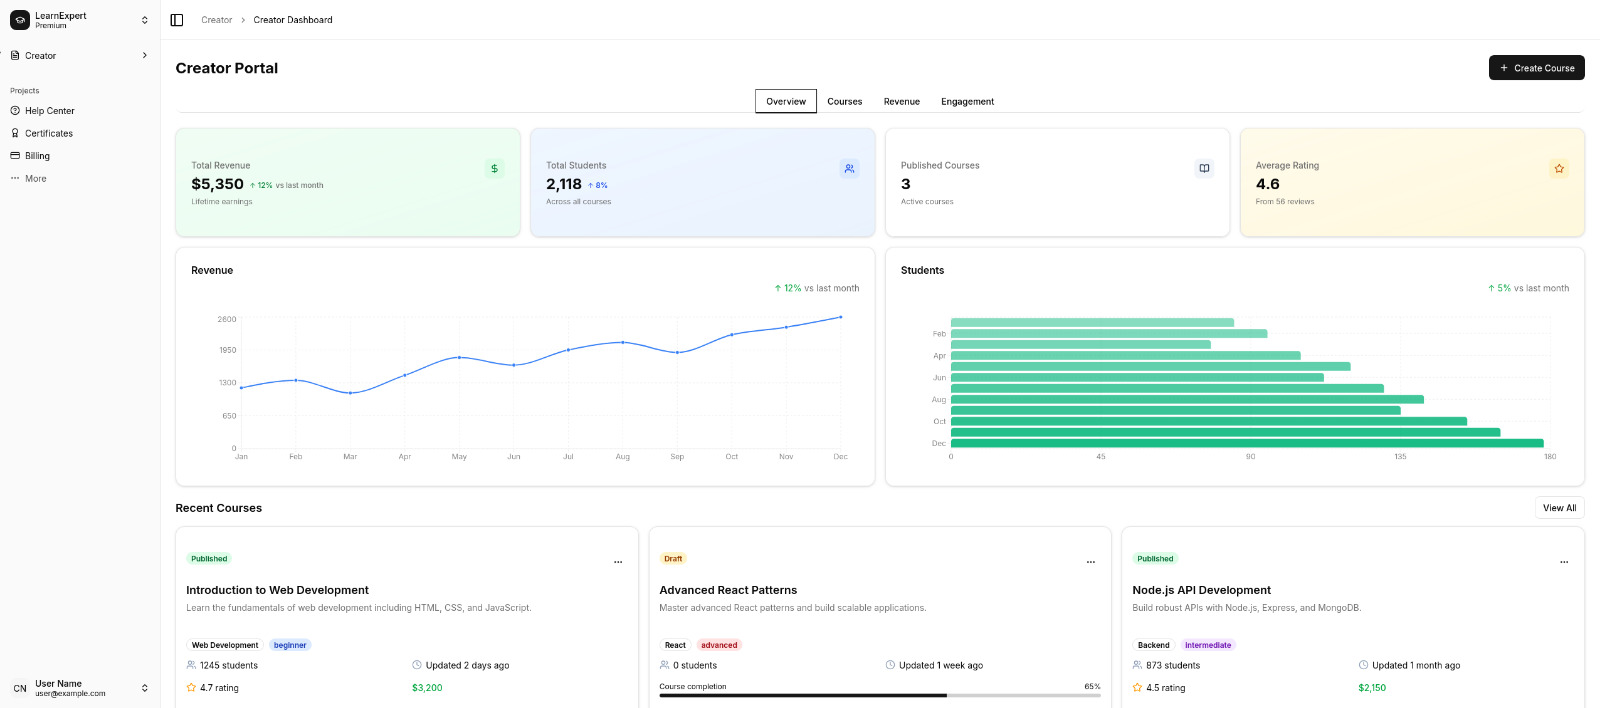
\includegraphics[width=0.85\textwidth]{cdash.jpeg} 
  \caption{Tableau de bord principal pour les créateurs de cours (Creator Portal).}
  \label{fig:creator_dashboard}
\end{figure}

\subsubsection{Page d'Analyse des Cours (Creator Analytics)}
Une page dédiée aux analyses détaillées a été implémentée, permettant aux créateurs de suivre l'engagement des étudiants. Elle présente des métriques telles que le temps de visionnage, les tentatives de quiz et les commentaires, avec des visualisations graphiques (combinées, linéaires, barres) pour faciliter l'interprétation des données. (Voir Figure \ref{fig:creator_analytics}).

\begin{figure}[htbp]
  \centering
  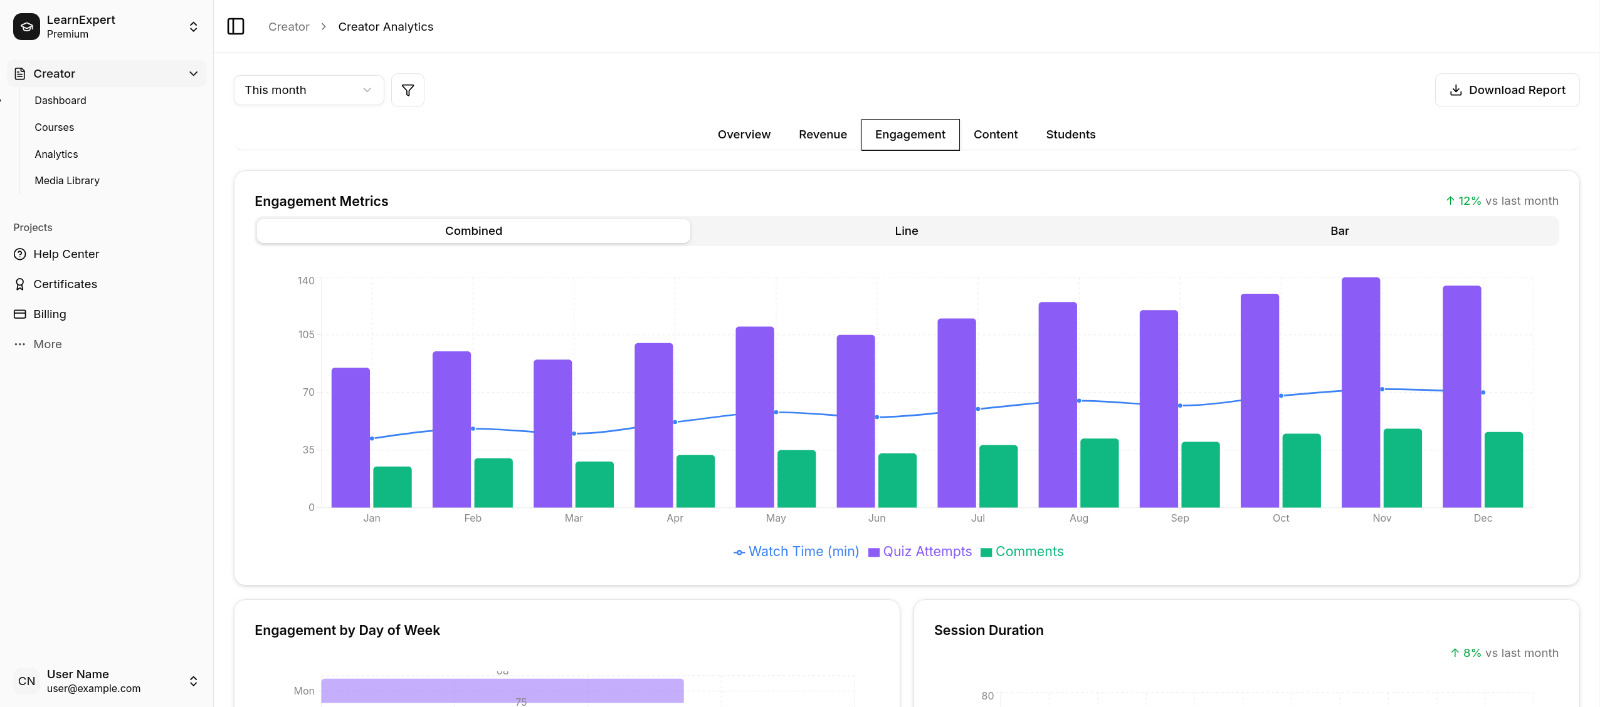
\includegraphics[width=0.85\textwidth]{analytics.jpeg} 
  \caption{Page d'analyse de l'engagement pour les créateurs.}
  \label{fig:creator_analytics}
\end{figure}

\subsubsection{Gestion des Cours et Logique de Création (Your Courses)}
L'interface de gestion des cours ("Your Courses") a été mise en place. Elle affiche les cours publiés et les brouillons, avec des statistiques clés par cours. Des fonctionnalités de recherche et de filtrage ont été intégrées, ainsi qu'un point d'entrée pour la création de nouveaux cours (bouton "Create Course"), initiant ainsi le développement de la logique de création de cours. (Voir Figure \ref{fig:creator_courses}).

\begin{figure}[htbp]
  \centering
  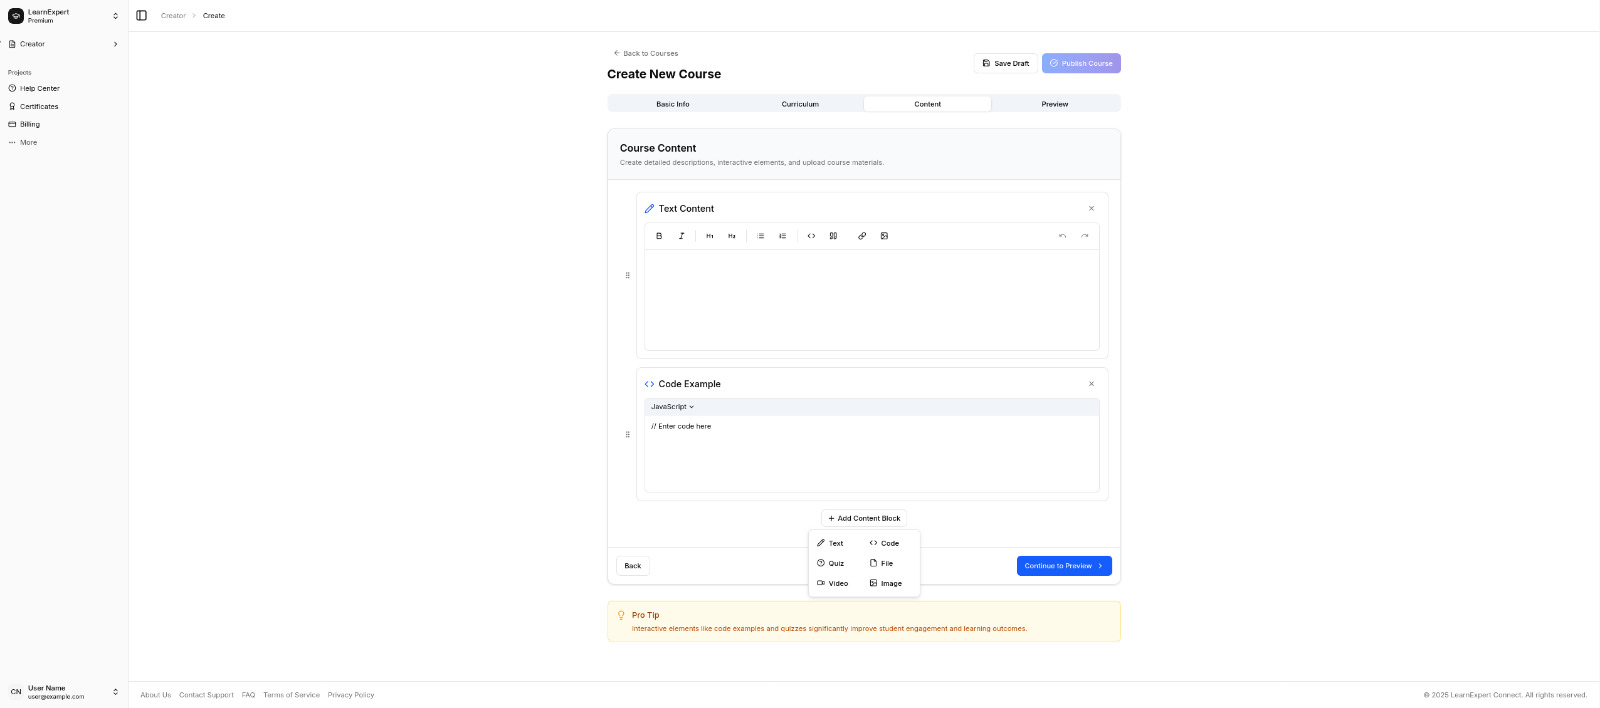
\includegraphics[width=0.85\textwidth]{create_course.jpeg} 
  \caption{Interface de gestion des cours pour les créateurs, incluant l'accès à la création de cours.}
  \label{fig:creator_courses}
\end{figure}

\subsection{Développement des Interfaces Côté Administrateur}
Le travail sur la section administrative de la plateforme a également progressé.

\subsubsection{Tableau de Bord Administrateur}
Le tableau de bord administrateur a été finalisé. Il fournit un aperçu global de la plateforme, affichant des indicateurs clés tels que le nombre total d'utilisateurs, les entreprises actives, les inscriptions aux cours et les revenus de la plateforme. Il inclut également des alertes importantes (charge serveur, demandes de vérification, contenu à modérer) et un résumé des actions en attente. (Voir Figure \ref{fig:admin_dashboard}).

\begin{figure}[htbp]
  \centering
  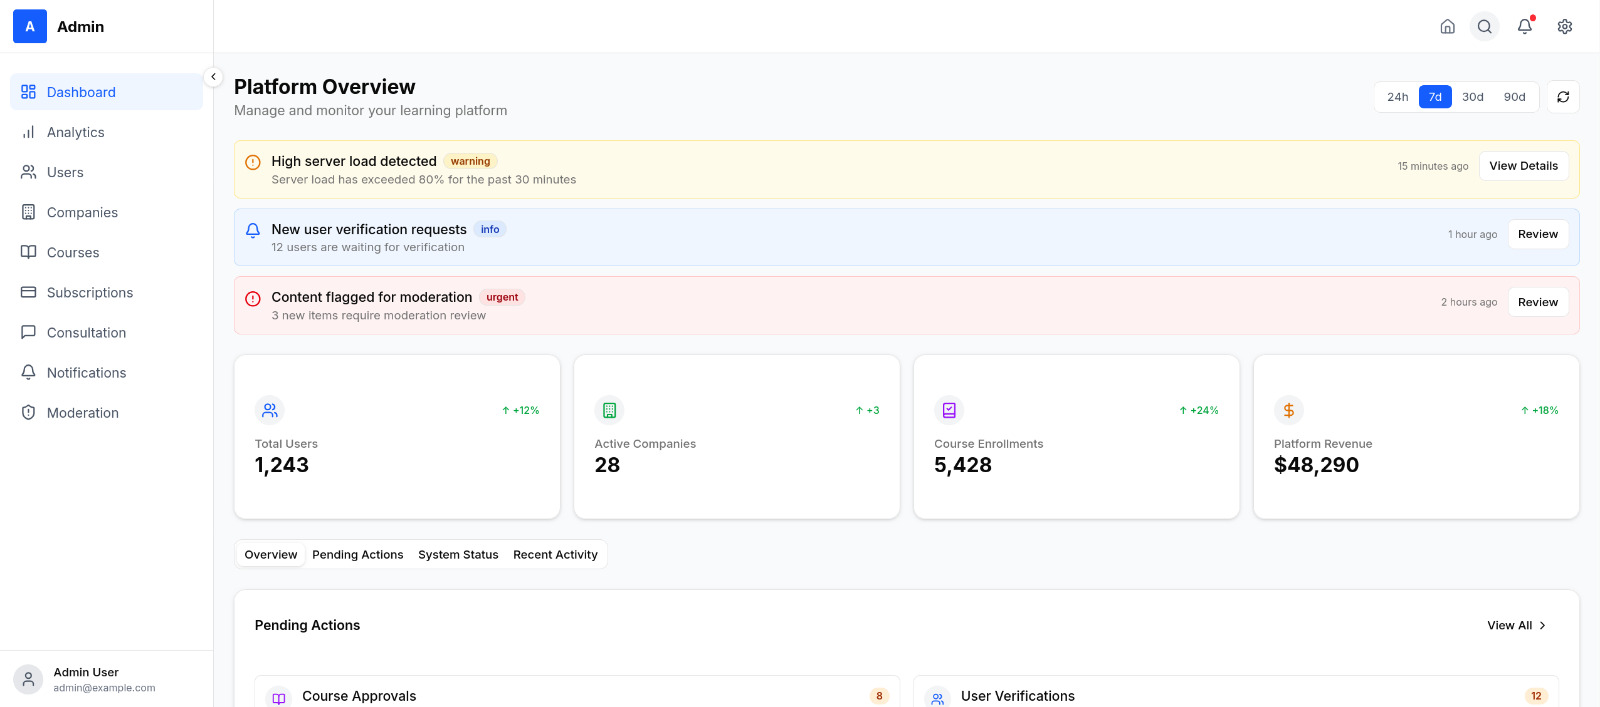
\includegraphics[width=0.85\textwidth]{admin.jpeg} 
  \caption{Tableau de bord de l'administrateur de la plateforme.}
  \label{fig:admin_dashboard}
\end{figure}

\subsubsection{Autres Pages Administrateur (En Cours)}
Le développement des autres pages de la section administrateur (gestion des utilisateurs, des entreprises, des cours, des abonnements, modération, etc.) a été initié. Bien qu'elles ne soient pas encore complètes à 100\%, les structures de base et les principaux composants UI sont en cours d'implémentation.

\subsection{Planification pour le Jour Suivant (Vendredi 30 Mai 2025)}
Pour la journée de demain, les activités prévues sont :
\begin{itemize}
  \item Finaliser le développement des interfaces restantes pour la section administrateur.
  \item Commencer la conception et l'implémentation des pages d'authentification (connexion, inscription, récupération de mot de passe).
  \item Débuter la phase de planification détaillée pour le développement backend et l'intégration des fonctionnalités principales de la plateforme.
\end{itemize}

\section{Conclusion}
Cette journée a permis de réaliser des avancées majeures dans la construction des interfaces pour les créateurs de cours et les administrateurs de LearnExpert. Les tableaux de bord, les outils d'analyse et les interfaces de gestion des cours fourniront des fonctionnalités essentielles pour ces deux rôles clés. La finalisation du tableau de bord administrateur est une étape importante, et les travaux sur les autres sections administratives progressent bien. Demain, l'accent sera mis sur l'achèvement de ces interfaces et sur la transition vers les aspects d'authentification et la planification du backend.

\end{document}